\documentclass[a4paper, 12pt]{article}

\usepackage[T1]{fontenc}
\usepackage{breakurl}
\usepackage[czech]{babel}
\usepackage[top=2.5cm,bottom=2.5cm,left=3.5cm,right=2.5cm]{geometry}
\usepackage[scaled=1]{helvet}
\usepackage{graphicx}
\usepackage[dvipsnames]{xcolor} % for colored text
\usepackage[colorlinks=true, allcolors=RoyalBlue]{hyperref}
\usepackage{tocloft} % Table of contents
\usepackage{multicol} % Multiple columns
\usepackage{wrapfig}
\usepackage{index}
\usepackage{courier} % Sets font for listing as Courier.
\usepackage{listings, xcolor}
\usepackage{tcolorbox}
\usepackage{subfig}
\usepackage{setspace}
\usepackage{titlesec}
\usepackage{todonotes}
\usepackage{csquotes}
\usepackage{filecontents} % data or code snippets from external sources
\usepackage{microtype} % Zlepší dělení a vizuální výstup



% Sections on new page
\newif\ifclearpageenabled
\clearpageenabledtrue % Set the variable to true by default
\AddToHook{cmd/section/before}{
    % Check if \clearpageenabled is true
    \ifclearpageenabled
        \clearpage % Execute \clearpage if true
    \fi
}




% Ukázky kódu
\renewcommand\lstlistlistingname{\LARGE Seznam ukázek kódu}
\renewcommand\lstlistingname{Ukázka}
\definecolor{backcolour}{rgb}{0.95,0.95,0.97}
\lstdefinestyle{Python}{
    language=Python,
    basicstyle=\scriptsize\fontfamily{lmtt}\selectfont,
    backgroundcolor=\color{backcolour},
    keywordstyle=\color{blue},
    commentstyle=\color{green!40!black},
    stringstyle=\color{RedViolet},
    showstringspaces=false,
    breaklines=true,
    breakatwhitespace=true,
    tabsize=4,
    numbers=left,
    numberstyle=\tiny\color{gray},
    frame=single,
    columns=fullflexible,
    % rulecolor = \color{black}, %% set frame color to avoid being affected by text color
}
\lstdefinestyle{bash}{
    language=bash,
    basicstyle=\ttfamily\footnotesize,
    keywordstyle=\color{blue},
    commentstyle=\color{gray},
    stringstyle=\color{red},
    backgroundcolor=\color{lightgray!20},
    frame=single,
    breaklines=true,
    postbreak=\mbox{\textcolor{red}{$\hookrightarrow$}\space},
}

\lstdefinelanguage{JavaScript}{
  keywords={typeof, new, true, false, catch, function, return, null, catch, switch, var, if, in, while, do, else, case, break, const},
  keywordstyle=\color{blue}\bfseries,
  ndkeywords={class, export, boolean, throw, implements, import, this},
  ndkeywordstyle=\color{darkgray}\bfseries,
  identifierstyle=\color{black},
  sensitive=false,
  comment=[l]{//},
  morecomment=[s]{/*}{*/},
  commentstyle=\color{purple}\ttfamily,
  stringstyle=\color{red}\ttfamily,
  morestring=[b]',
  morestring=[b]"
}

\lstdefinestyle{JavaScript}{
    language=JavaScript,
    basicstyle=\scriptsize\fontfamily{lmtt}\selectfont,
    backgroundcolor=\color{backcolour},
    keywordstyle=\color{blue},
    commentstyle=\color{green!40!black},
    stringstyle=\color{RedViolet},
    showstringspaces=false,
    breaklines=true,
    breakatwhitespace=true,
    tabsize=4,
    numbers=left,
    numberstyle=\tiny\color{gray},
    frame=single,
    columns=fullflexible,
    % rulecolor = \color{black}, %% set frame color to avoid being affected by text color
}


\lstdefinelanguage{XML_SYNTAX}{%
    alsoletter=-,
    morestring=[b]",stringstyle=\color[rgb]{0,0,1},
    moredelim=*[s][{\color[rgb]{0.75,0,0}}]{<}{>},
    moredelim=[s][{\color[rgb]{0,0,0}}]{<!--}{-->},
    moredelim=[s][{\color[rgb]{0,0.75,0}}]{\ }{=},
    moredelim=[s][{\color[rgb]{0,0.75,0}}]{\    }{=} % here there is \tab
}

\lstdefinestyle{HTML}{
    % Basic design
    backgroundcolor=\color{backcolour},
    basicstyle=\scriptsize\fontfamily{lmtt}\selectfont,
    breaklines=true,
    frame=l,
    tabsize=4,    
    breakatwhitespace=true,
    numbers=left,    
    numberstyle=\tiny\color{gray},
    frame=single,
    numberfirstline=true,
    % HTML formatting
    language=XML_SYNTAX,
}

\lstdefinelanguage{CSS}{
  keywords={background-color, height, width, border, radius, animation, opacity, position, z, index, background, color, transform, left, top, margin, padding, overflow, backdrop, filter, box, shadow, webkit, transition},
  keywordstyle=\color{blue}\bfseries,
  ndkeywords={ ease, in, out, infinite, both, alternate, var, px, rem, s},
  ndkeywordstyle=\color{green!50!black}\bfseries,
  identifierstyle=\color{orange}\bfseries,
  sensitive=false,
  comment=[l]{/*},
  morecomment=[s]{/*}{*/},
  commentstyle=\color{purple}\ttfamily,
  stringstyle=\color{red}\ttfamily,
  morestring=[b]',
  morestring=[b]"
}

\lstdefinestyle{CSS}{
    language=CSS,
    basicstyle=\scriptsize\fontfamily{lmtt}\selectfont,
    backgroundcolor=\color{backcolour},
    keywordstyle=\color{blue},
    commentstyle=\color{green!40!black},
    stringstyle=\color{RedViolet},
    showstringspaces=false,
    breaklines=true,
    breakatwhitespace=true,
    tabsize=4,
    numbers=left,
    numberstyle=\tiny\color{gray},
    frame=single,
    columns=fullflexible,
    % rulecolor = \color{black}, %% set frame color to avoid being affected by text color
}



% List of figures
\renewcommand{\cftloftitlefont}{\LARGE\bfseries}
\renewcommand\cftfigfont{\small}
\renewcommand\cftfigpagefont{\small}


% Bibliography
\usepackage[natbib=true,
    style=numeric,
    sorting=none]{biblatex}
\addbibresource{ref.bib}
% Define a command to set the font size for the bibliography entries
\newcommand{\setbibfont}{\small} 
\AtBeginBibliography{\setbibfont}



%% Section font format
\titleformat*{\section}{\LARGE\bfseries}
\titleformat*{\subsection}{\Large\bfseries}
\titleformat*{\subsubsection}{\large\bfseries}
\titleformat*{\paragraph}{\large\bfseries}
\titleformat*{\subparagraph}{\large\bfseries}


\setstretch{1.5}
\hyphenpenalty=10000\exhyphenpenalty=10000 %žádné pomlčky na konci
\setlength {\marginparwidth }{2cm} 


\begin{document}



\pagenumbering{gobble} %%no page number

\renewcommand{\cftsecleader}{\cftdotfill{\cftdotsep}}
\title{\textbf{Maturitní práce}}

\author{} %fix alert
\maketitle

\centerline{\Large {\textbf{ Gymnázium, Praha 6, Arabská 14}} \par}
\centerline{ \large    Arabská 14, Praha 6, 160 00 \par} 
\begin{figure}[hp]
    \centering
    
\includegraphics[scale = 0.5]{Images/GA_logo.png}
    
\end{figure}

\vfill
\begin{flushleft}
\textbf{Předmět:} Programování\newline
\textbf{Téma:} Nástroj pro tvorbu myšlenkových map  \newline
\newline
\textbf{Autor:} \author{\textit{Vítězslav Procházka}} \newline
\textbf{Třída:} 4.E  \newline
\textbf{Vyučující:} Mgr. Jan Lána \newline
\textbf{Tř. vyučující:} Mgr. Blanka Hniličková

\end{flushleft}
% Turn off \clearpage for specific pages
\clearpageenabledfalse % Disable \clearpage
\newpage


\mbox{}
\vfill
\begin{Large}
\section*{Čestné prohlášení:}
\end{Large}
\par Prohlašuji, že jsem jediným autorem tohoto projektu, všechny citace jsou řádně označené a všechna použitá literatura a další zdroje jsou v práci uvedené. 
\par Tímto dle zákona 121/2000 Sb. (tzv. Autorský zákon) ve znění pozdějších předpisů uděluji bezúplatně škole Gymnázium, Praha 6, Arabská14 oprávnění k výkonu práva na rozmnožování díla (§ 13) a práva na sdělování díla veřejnosti (§ 18) na dobu časově neomezenou a bez omezení územního rozsahu.

\vspace{40pt}
\noindent
V Praze dne …………………… \hspace{20pt} …………………… \\


\clearpageenabledtrue % Re-enable \clearpage for subsequent pages
\clearpageenabledfalse % Disable \clearpage
\newpage
\mbox{}
\vfill
\section*{Poděkování}
Chtěl bych poděkovat Mgr. Janu Lánovi za vedení této práce.
Dále bych chtěl poděkovat Mgr. Jiřímu Procházkovi za pomoc při navrhování ovládání a jeho následné testování . Velké díky také patří Ing. Václavu Chalupníčkovi za velmi srozumitelný úvod do tvorby webových aplikací.

\clearpageenabledtrue



\section *{Anotace}

\clearpageenabledfalse % Disable \clearpage

Tato dokumentace popisuje maturitní práci, na téma: Nástroj pro tvorbu myšlenkových map.
Cílem tohoto projektu je vytvořit intuitivní nástroj pro tvorbu myšlenkových map v podobě webové stránky. Každý uživatel bude mít svůj vlastní workspace, kde bude mít online uložené své vlastní privátní myšlenkové mapy. Myšlenkové mapy by měly jít snadno vytvářet a upravovat. Dalším podstatným prvkem je přehlednost uživatelského rozhraní. 
\section *{Klíčová slova}
Myšlenková mapa; ; webová aplikace; graf; brainstorming; organizace myšlenek;

\vspace{40pt}
\section*{Abstract (English)}
This documentation describes a year-end project on the topic: A Tool for Creating Mind Maps.
The goal of this project is to create an intuitive tool for mind map creation in the form of a website. Each user will have their own workspace, where they can store their private mind maps online. Mind maps should be easy to create and edit. Another essential element is the clarity of the user interface.

\section *{Keywords}
Mind map; web application; graph; brainstorming; thoughts organization;


\clearpageenabledtrue 


\newpage
\pagenumbering{arabic} % start numbering pages
% \linespread{0.9}\selectfont
\tableofcontents
% \linespread{1.5}\selectfont
\section{Úvod}
Myšlenkové mapy představují efektivní nástroj pro vizualizaci a organizaci informací, podporující kreativní myšlení, analýzu problémů a strukturování myšlenek. Jejich využití se rozšířilo do různých oblastí, včetně vzdělávání, projektového řízení, vědeckého výzkumu a osobního rozvoje. Tradičně se myšlenkové mapy vytvářely na papíře, avšak s rozvojem digitálních technologií se stále více uplatňují webové aplikace umožňující dynamickou práci s uzly, propojeními a interaktivními prvky.
\newline

Tato práce se zaměřuje na návrh a implementaci webové aplikace pro tvorbu myšlenkových map, která poskytuje uživatelům intuitivní rozhraní pro vytváření a editaci myšlenkových schémat. Cílem je vytvořit prototyp webové aplikace, která přináší přehledné, čisté uživatelské rozhraní a snadné, zapamatovatelné ovládání.
\newline

Projekt je stavěn na moderních  technologiích pro vývoj webových aplikací, včetně frameworků pro dynamické uživatelské rozhraní a nástrojů pro práci s grafovými strukturami a jejich vizualizaci.
\newline

Jméno projektu Idea-Atlas (z angličtiny: atlas idejí) má vyjadřovat účel projektu; tedy mapovat ideje (myšlenky).

\begin{figure}[h]
    \centering
    \includegraphics[width=0.3\linewidth]{Images/Logo.png}
    \caption{Logo Idea-Atlas}
\end{figure}
\newpage
\subsection{Zadání projektu}
IdeaAtlas bude online webový nástroj pro tvorbu myšlenkových map. Uživatelům umožní jednoduše uspořádat své myšlenky a nápady do grafů závislostí mezi pojmy. Uživatelé budou moci přidávat nové položky, měnit jejich vztahy, mazat je, a tím upravovat myšlenkovou mapu. Další funkcí tohoto nástroje bude generování souvislostí a pojmů pomocí ChatGPT. Každý uživatel bude mít svůj vlastní workspace, což znamená, že jeho mapy budou uloženy na serveru. Tento nástroj bude ideální pro brainstorming a vizualizaci souvislostí libovolné problematiky.
\subsection{Důvod výběru tématu}
Vybral jsem si téma nástroj pro tvorbu myšlenkových map, protože mě zaujal koncept vizuálního mapování nápadů a jejich propojení do dynamické struktury. Zároveň mi téma přišlo obtížné, nikoliv však nemožné. Práce s grafy, interaktivní vizualizací a databázemi přináší spoustu výzev. Dále jsem si chtěl vyzkoušet moderní technologie pro tvorbu webových aplikací a prozkoumat, jak je lze efektivně kombinovat.
\section{Použité technologie}
V mém projektu jsme se rozhodl využít tyto programovací jazyky, frameworky a významné knihovny.
\begin{enumerate}
    \item Nuxt 3 - full stack framework\cite{Nuxt}
    \begin{itemize}
        \item Vue.js - front-end framework na kterém staví Nuxt\cite{Vue}
        \item V-network-graph - knihovna pro tvorbu relačníh interaktivních grafů\cite{VNetwork}
        \end{itemize}
    \item JavaScript, TypeScript – Logika uživatelského rozhraní, dotazy do databáze
        \begin{itemize}
        \item D3.js - Knihovna pro tvorbu grafů (v mé práci použita k implementaci force layout) \cite{D3}
        \end{itemize}
    \item Supabase - open source alternativa k firebase, databáze, Baas (back-end as service)\cite{Supabase}
    \item Tailwind CSS - jednodušší a organizovaný design UI\cite{TailwindNuxt}
    \item Bun - rychlejší alternativa k Node.js; runitme, package manage, bundler \cite{bun}
        
\end{enumerate}

\section{Brainstorming a myšlenkové mapy}

V dnešním světě, kde inovace hrají klíčovou roli, je schopnost generovat nové nápady zásadní. Existuje mnoho metod, jak podpořit kreativní myšlení, ale dvě z nejefektivnějších jsou brainstorming a myšlenkové mapy. Tyto techniky nejen usnadňují proces tvorby nápadů, ale také pomáhají organizovat myšlenky do srozumitelných struktur.\cite{brainstorming3}

\subsection{Brainstorming: Svoboda Myšlení}
Brainstorming je oblíbená metoda, která umožňuje jednotlivcům i skupinám přicházet s novými nápady bez obav z okamžitého hodnocení. Tento proces podporuje volné myšlení a často vede k překvapivým a inovativním řešením. Základní pravidlo brainstormingu spočívá v tom, že neexistují špatné nápady – jakýkoliv návrh může sloužit jako inspirace pro další myšlenky.\cite{brainstorming1}
\newline

Brainstorming obvykle probíhá v několika fázích. Nejprve je definován problém nebo téma, na které se skupina soustředí. Poté účastníci spontánně sdílejí své myšlenky, aniž by byly okamžitě analyzovány nebo kritizovány. Teprve v závěrečné fázi dochází k selekci a hodnocení nápadů s cílem vybrat ty nejefektivnější. Tento přístup eliminuje bariéry v myšlení a umožňuje vznik inovativních konceptů, které by jinak mohly být přehlédnuty.\cite{brainstorming2}

\subsection{Myšlenkové Mapy: Strukturované Myšlení}
Zatímco brainstorming podporuje rychlý tok nápadů, myšlenkové mapy slouží k jejich vizualizaci a organizaci. Myšlenková mapa je grafické znázornění informací, které propojuje jednotlivé pojmy a ukazuje jejich vzájemné vztahy. Tato metoda je velmi efektivní nejen při plánování projektů, ale také při učení nebo řešení složitých problémů.
\newpage
Vytvoření myšlenkové mapy začíná ústředním pojmem, který je umístěn do středu diagramu. Od něj se větví hlavní témata, která se dále dělí na podtémata. Tento proces napodobuje přirozený způsob, jakým mozek zpracovává informace, což z něj činí intuitivní a účinný nástroj.

Používání myšlenkových map pomáhá lépe pochopit složité souvislosti a usnadňuje zapamatování informací. Díky své vizuální podobě umožňují snadnější orientaci v nápadech a podporují kreativní řešení problémů. \cite{mindmapscom-2021}

\subsection{Propojení Brainstormingu a Myšlenkových Map}
Brainstorming a myšlenkové mapy se vzájemně doplňují. Po ukončení brainstormingu je možné převést výsledné nápady do myšlenkové mapy, což pomůže s jejich organizací a dalším rozpracováním. Tento postup umožňuje nejen efektivnější řízení kreativního procesu, ale také lepší pochopení a využití generovaných myšlenek.
\newline

V dnešní době, kdy jsou kreativita a inovace nezbytné pro úspěch, jsou tyto techniky cenným nástrojem pro každého, kdo se snaží přicházet s novými nápady a hledat neotřelá řešení. Ať už pracujeme na osobních projektech, nebo spolupracujeme v týmu, brainstorming a myšlenkové mapy nám pomáhají překonat bariéry v myšlení a nacházet nové perspektivy. \cite{brainstorming3, mindmapscom-2020}
\section{Instalace}
\subsection{Linux Setup}

Pro správnou instalaci projektu IdeaAtlas na operační systém Linux postupujte podle následujících kroků:

\textbf{Klonování repozitáře}
\newline
Nejprve naklonujte repozitář pomocí příkazu:

\begin{lstlisting}[style= bash]
git clone https://github.com/gyarab/2024-4e-prochazka-IdeaAtlas.git
\end{lstlisting}

\textbf{Instalace Bun}
\newline
Nainstalujte správce balíčků Bun spuštěním následujícího příkazu:

\begin{lstlisting}[style= bash]
curl -fsSL https://bun.sh/install | bash
\end{lstlisting}

\textbf{Přechod do adresáře projektu}
\newline
Přejděte do hlavního adresáře projektu:

\begin{lstlisting}[style= bash]
cd 2024-4e-prochazka-IdeaAtlas
cd idea-atlas
\end{lstlisting}

\textbf{Instalace závislostí}
\newline
Nakonec nainstalujte všechny závislosti projektu:

\begin{lstlisting}[style= bash]
bun install
\end{lstlisting}

Po úspěšném dokončení těchto kroků by měl být projekt připraven k použití.

\newpage
\subsection{Widnows setup}
Pro správnou instalaci projektu IdeaAtlas na operační systém Windows postupujte podle následujících kroků:

\textbf{Klonování repozitáře}
\newline
Nejprve naklonujte repozitář pomocí příkazu:

\begin{lstlisting}[style= bash]
git clone https://github.com/gyarab/2024-4e-prochazka-IdeaAtlas.git
\end{lstlisting}
\textbf{Instalace Bun}
\newline
Nainstalujte správce balíčků Bun spuštěním následujícího příkazu:

\begin{lstlisting}[style= bash]
powershell -c "irm bun.sh/install.ps1 | iex"
\end{lstlisting}

\textbf{Přechod do adresáře projektu}
\newline
Přejděte do hlavního adresáře projektu:

\begin{lstlisting}[style= bash]
cd 2024-4e-prochazka-IdeaAtlas
cd idea-atlas
\end{lstlisting}

\textbf{Instalace závislostí}
\newline
Nakonec nainstalujte všechny závislosti projektu:

\begin{lstlisting}[style= bash]
bun install
\end{lstlisting}

Po úspěšném dokončení těchto kroků by měl být projekt připraven k použití.


\subsection{Spuštění projektu}
Pro spuštění projektu: v adresáři \textit{2024-4e-prochazka-IdeaAtlas\textbackslash idea-atlas} použijte příkaz
\begin{lstlisting}[style= bash]
bun run dev
\end{lstlisting}
\section{Ovládání}
Ovládání výrazně závisí na klávesových zkratkách, nástroj tedy není vhodný k používání na mobilu. Snažil jsem se, aby ovládání bylo intuitivní a lehce se dalo zapamatovat. Seznam všech zkratek naleznete v kapitole \ref{seznam}
\subsection{Pohyb po myšlenkové mapě}
Pokud zmáčkneme levé tlačítko (do prázdného prostoru) a budeme ho držet, můžeme myšlenkovou mapou pohybem myši posouvat. Pro přibližování a oddalování slouží kolečko na myši.
\subsection{Přidání nového vrcholu}
Pro přidání nového vrcholu stačí namířit myšítkem na zvolené místo pro nový vrchol. Dvojklikněme levým tlačítkem myši nebo stiskněme klávesu Enter pro zobrazení dialogu pro tvorbu nového vrcholu (obrázek \ref{fig:input}. Zde vyplňme jméno, zvolme barvu a velikost. Tento dialog se dá posouvat za jeho záhlaví a pro jeho zmizení stačí kliknout mimo něj.
\begin{figure}[h]
    \centering
    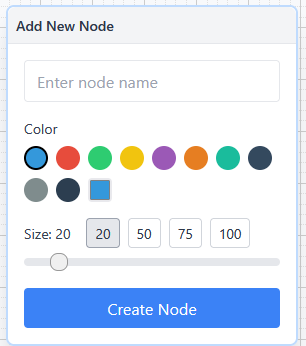
\includegraphics[width=0.5\linewidth]{Images/inputdialog.png}
    \caption{Dialog pro přidání nového vrcholu}
    \label{fig:input}
\end{figure}
\subsection{Selekce vrcholů a hran}
Existuje hned několik způsobů, jak vybrat prvky. Pro vybrání jedné hrany nebo vrcholu na ně stačí kliknout levým tlačítkem myši. Pokud jich chceme vybrat více, musíme u toho držet \textit{LShift}.
\par
Dále můžeme hrany vybrat pomocí obdélníkového výběru, který aktivujeme klávesou \textit{Ctrl} a tažením myši při držení stisknutého levého tlačítka, viz obrázek \ref{fig:select}.
\begin{figure}[h]
    \centering
    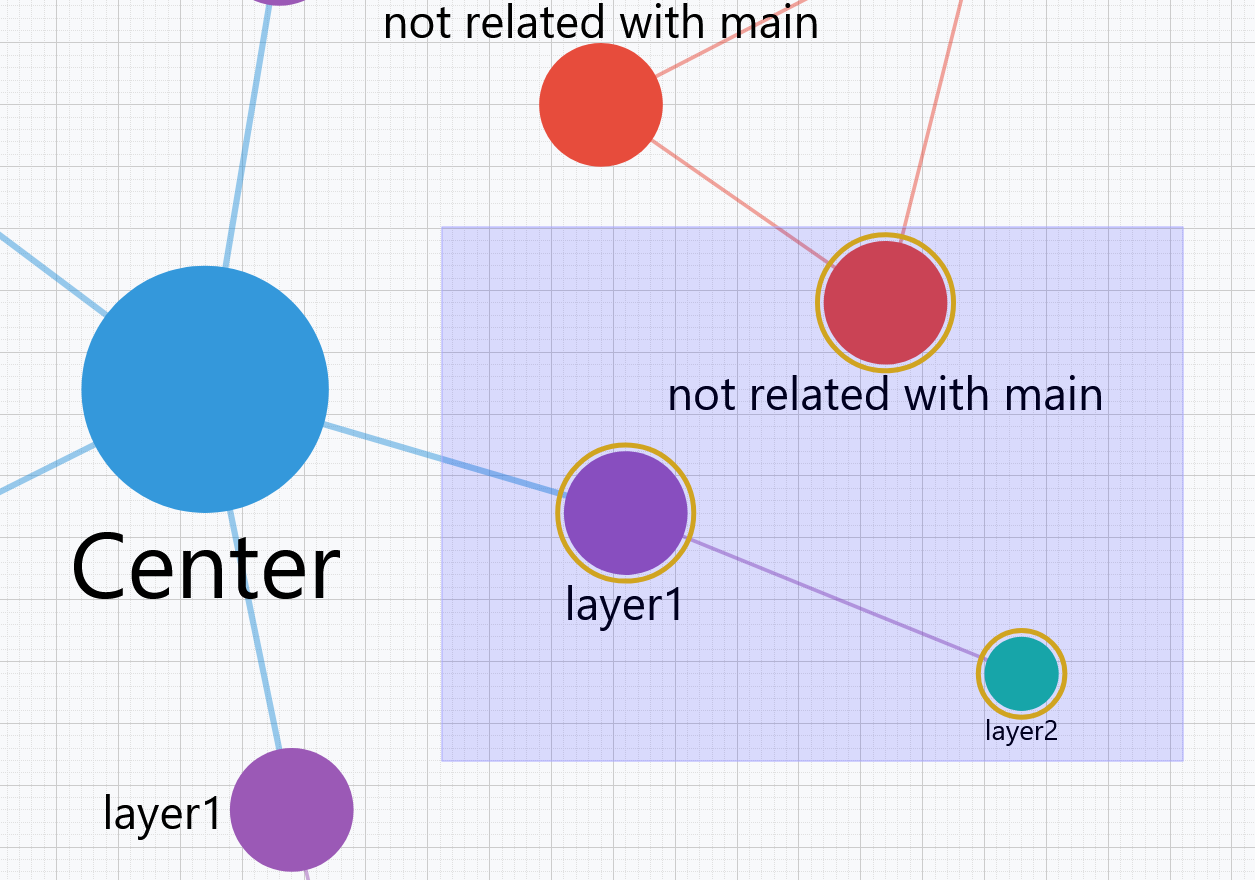
\includegraphics[width=0.5\linewidth]{Images/select.png}
    \caption{Obdélník pro selekci vrcholů}
    \label{fig:select}
\end{figure}
\par
Další speciální způsob, jak označit vrcholy, je pomocí \textit{wave selectu}, který postupně rekurzivně označí vrcholy spojené s těmi již označenými. Vždy je zde časová prodleva, než se vybere další vrstva, postupně je tato prodleva snižována; pro případy, kdy chce uživatel takto označit velké množství vrcholů. Selekce probíhá, pokud uživatel drží klávesu \textit{W}, pokud ji pustí, dojde k přerušení a další vrcholy nebudou vybrány. Tato funkcionalita se zejména hodí, pokud naše myšlenková mapa má strukturu lesa, má tedy hodně oddělených stromů - jednoduše se tak dá vybrat právě jeden celý strom.
\par
Poslední způsob, jak vybrat vrcholy, je pomocí vyhledávání. Automaticky se budou vybírat ty vrcholy, které obsahují zadaný řetězec.
\par
Pro odznačení jakéhokoliv výběru stačí kliknout levým tlačítkem myši na pozadí.
\newpage
\subsection{Přidání hran mezi vrcholy}
Pokud máme označené dva vrcholy, pomocí mezerníku je spojíme. Pokud máme označeny 3 nebo více vrcholů, po zmáčknutí mezerníku se spojí všechny vybrané vrcholy s tím, co bylo označeno jako první. Pokud chceme spojit všechny vrcholy mezi sebou, stačí zmáčknout najednou \textit{Ctrl} a mezerník.

\subsection{Odebrání vrcholu a hran}
Po stisknutí klávesy \textit{backspace} dojde k smazání vybraných prvků, nezáleží na tom, jestli jde o hrany nebo vrcholy. Pokud ovšem chceme smazat hrany, které mezi sebou sdílí vybrané vrcholy, dosáhneme toho tím stisknutím \textit{ctrl} a \textit{backspace}.
\subsection{Úprava vrcholu}
Pro úpravu vrcholu na něj dvojklikněme levým tlačítkem myši nebo pomocí klávesové kombinace \textit{ctrl} a \textit{Enter}. Objeví se nám dialog pro úpravu vrcholu (obrázek \ref{fig:edit}), který je předvyplněný jeho aktuálními parametry. Tento dialog se dá posouvat za jeho záhlaví a pro jeho zmizení stačí kliknout mimo něj.
\begin{figure}[h]
    \centering
    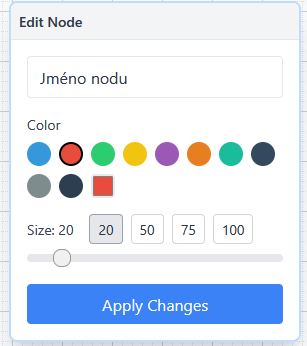
\includegraphics[width=0.5\linewidth]{Images/style.png}
    \caption{Dialog pro úpravu vrcholu}
    \label{fig:edit}
\end{figure}
\subsection{Undo a Redo}
Pro odčinění poslední akce stiskněte klávesovou kombinaci \textit{Ctrl} a \textit{Z}. Pokud jsme se vrátili o pár akcí do minulosti v historii provedených kroků, můžeme se pohybovat zpět k současnému bodu pomoci kombinace kláves \textit{Ctrl}, \textit{LShift} a \textit{Z}
\subsection{Změna layoutu}
Pomocí tlačítka Force Layout a Grid Layout (záleží, co je aktuálně vybráno) můžeme tyto dva režimy přepínat.
\subsection{Uložení}
Pro uložení neslouží žádná klávesová zkratka, ale tlačítko Save. Nebo stačí, pokud nebudeme dělat žádné změny po dobu delší než 2 vteřiny. 
\subsection{Seznam všech klávesových zkratek}
\label{seznam}
Veškeré klávesové zkratky naleznete na obrázku \ref{fig:shortcuts}; samotná webová stránka nabízí možnost zobrazení této nápovědy.
\begin{figure}[h]
    \centering
    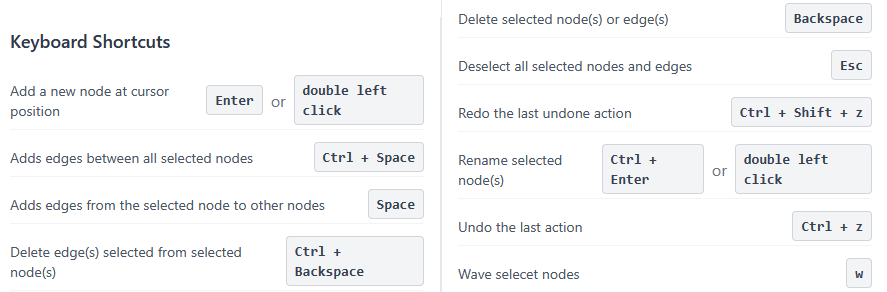
\includegraphics[width=1.1\linewidth]{Images/shortcuts.png}
    \caption{Seznam klávesových zkratek}
    \label{fig:shortcuts}
\end{figure}

\section{Frontend}
Webová aplikace je primárně postavena na Vue.js, moderní JavaScriptové knihovně určené k tvorbě dynamických uživatelských rozhraní. Využívá komponentový přístup, který umožňuje rozdělit rozhraní na menší, znovu použitelné části, čímž usnadňuje správu kódu a zlepšuje čitelnost projektu. Tento přístup nejen zjednodušuje vývoj, ale také usnadňuje rozšiřování a údržbu aplikace, což je klíčové pro škálovatelnost projektu.
\subsection{Routování}
V Nuxtu funguje routování automaticky díky file-based routing, což znamená, že struktura souborů ve složce \textit{pages/} určuje URL adresy aplikace. Například soubor \textit{pages/index.vue} odpovídá domovské stránce \textit{/}, zatímco \textit{pages/about.vue} vytváří routu \textit{/about}. Pro dynamické parametry se používají hranaté závorky, takže soubor \textit{pages/blog/[id].vue} odpovídá cestě \textit{/blog/:id}, kde lze parametr id získat pomocí \textit{useRoute()}.\cite{routing}
\subsection{Komponenty}
Vue.js i Nuxt staví na technologii komponentů.
Komponenty umožňují rozdělit komplexní UI problémy do mnoha menších podproblémů; je to podobné jako například funkce nebo třídy v objektově orientovaném programování. Jednotlivé komponenty jsou samostatné .vue soubory ve složce \textit{components}, obsahují HTML šablony, JavaScriptový (popřípadě TypeScriptový) kód i CSS styly. Komponenty pomáhají modulárně strukturovat aplikaci, což vede k lepší čitelnosti a opětovné použitelnosti kódu.\cite{component} Dále bych chtěl podotknout, že Nuxt zajišťuje automatické importování komponent, není tedy potřeba je v každém souboru importovat manuálně. \cite{nuxt-auto-import}
\newline
\newline
Nejvýznamnějším komponentem v tomto projektu je \textit{MapNetwork.vue}. V tomto komponentu se do hromady skládá veškerá funkcionalita nástroje na tvorbu myšlenkových map. V jádru této komponenty stojí knihovna V-network-graph, která se stará o reprezentaci i zobrazování relačních grafů viz kapitola \ref{vizualizcemap}. Jsou zde napojeny další UI komponenty, jak funkce spravující grafovou strukturu, tak funkce dotazující do databáze. Dále jsou zde handlery na obsluhování klávesových zkratek.
\newline
Dalšími významnými komponenty jsou \textit{NodeInputDialog.vue} \textit{NodeEditDialog.vue}, tyto UI komponenty zprostředkovávají uživatelské rozhraní pro editace (případně tvorbu) jednotlivých nodů. 

\subsection{Design}
Idea-Atlas je proveden v jednoduchém, čistém stylu. Dominantními barvami jsou modrá, světle šedá a bílá. Snažil jsem se, aby uživatelské rozhraní působilo přehledně a moderně, ale nikoliv však rušivě. Schválně jsem se vyhnul komplikovaným designovým prvkům a animacím, protože to není předmětem této práce.
\par
Zde jsou vyobrazeny ukázky těch zajímavějších částí webové aplikace. Na obrázku \ref{fig:home} je k nalezení hero nadpis úvodní domovské stránky. Na něm bych vypíchnul minimalistický design pomocí gradientů a poklidnou jednoduchou animaci pohupování.\cite{glow}
\begin{figure}[h]
    \centering
    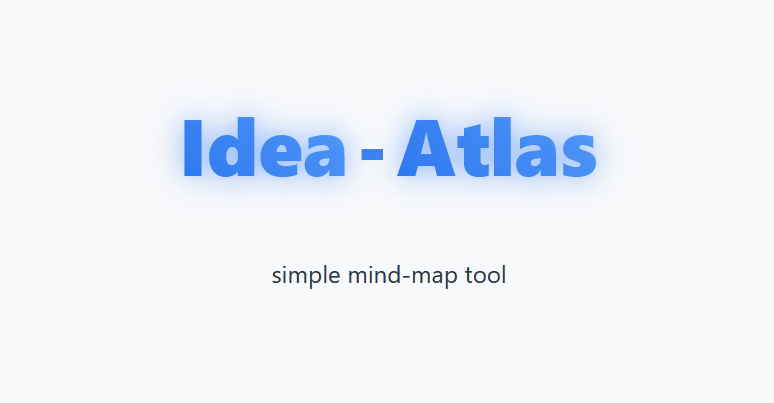
\includegraphics[width=0.9\linewidth]{Images/Homepage.png}
    \caption{Hero nadpis}
    \label{fig:home}
\end{figure}
\newpage
Na obrázku \ref{fig:card} je k vidění kartička jedné z map. Je na ní vidět, zda je bookmarknutá, kdy byla mapa vytvořena, kdy naposledy upravena, její jméno a popis.\cite{card} Dále jsou zde ikonky pro smazání dané mapy nebo upravení jejích metadat.
\begin{figure}[h]
    \centering
    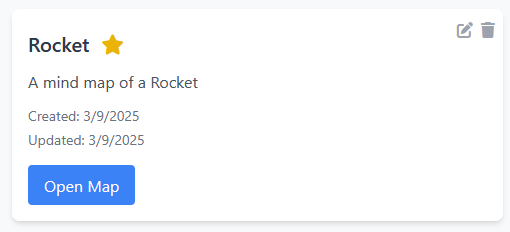
\includegraphics[width=1\linewidth]{Images/card.png}
    \caption{Kartička mapy}
    \label{fig:card}
\end{figure}

\section{Vizualizace myšlenkových map}
\label{vizualizcemap}
O zobrazování myšlenkových map se stará knihovna V-network-graph. Práce s ní byla vcelku přímočará, veškeré informace jsem čerpal z oficiální dokumentace s ukázkami \cite{vnetexamples}. Postupně jsem si z jednotlivých ukázek zaměřených vždy na jednu problematiku vybral, co potřebuji, a sestavil jsem z toho finální komplexní nástroj.
\newline
Samotná knihovna poskytuje následující funkce:
\begin{enumerate}
    \item zoom
    \item přesouvání se po mapě
    \item přidávání a odebírání vrcholu
    \item přidávání a odebírán hrany
    \item podpora customizace - barvy, velikosti, animace vrhcolů a hran
    \item dynamické překreslování (například při změně barvy vrcholu)
    \item interagování s grafem
    \item integrace force layoutu pomocí D3.js
    \item zobrazení mřížky
\end{enumerate}
\newpage
Jak již bylo zmíněno, vše dohromady přichází k "životu" v souboru \textit{MapNetwork.vue} . Veškerá funkcionalita a interaktivita s grafem je zřízena v souboru \textit{graphManager.js}, nacházející se zde funkce pro správu vrcholů, hran atd. Ukázka \ref{nodeadd} dává za příklad jednoduchou funkci pro přidání nového vrcholu. Vypočítá nové id a namapuje hodnoty pro nový vrchol. 
\begin{lstlisting}[style=JavaScript, firstnumber = 5, caption={utils/graphManager.js, přidání vrcholu do grafu},
label={nodeadd}]
// adds a new node to the graph
function addNewNode(data, nodeProps, xMousePos, yMousePos) {
    // Find the largest numeric part of the existing keys
    const maxNodeId = findCurrentMaxNodeId(data);
    // Generate the next key
    const nextNodeId = `node${maxNodeId + 1}`;
    
    // Add the new node with all properties
    data.nodes[nextNodeId] = {
        name: nodeProps.name,
        color: nodeProps.color,
        size: nodeProps.size
    };
    // Adds the new node to the layouts so its position is tracked
    data.layouts.nodes[nextNodeId] = { x: xMousePos, y: yMousePos };
    
    historyManager.addToHistory(data);
    
}
\end{lstlisting}
Nachází se zde ale i komplikovanější funkce, například \textit{waveNodeSelect} viz ukázka \ref{wave}. Tato funkce rekurzivně přidává vrcholy, které jsou potomky těch již označených, do označených vrcholů. Tato funkcionalita rozšiřuje možnosti editace myšlenkových map.
\newpage
\begin{lstlisting}[style=JavaScript, firstnumber = 264, caption={utils/graphManager.js, wave select},
label={wave}]
// Function which will recusively select all the nodes connected to the selected node
async function waveNodeSelect(data, selectedNodes, callback) {
    const visited = new Set(selectedNodes);
    const newlySelected = [];
    
    // Get connected nodes that haven't been visited
    Object.values(data.edges).forEach(edge => {
        const source = edge.source;
        const target = edge.target;
        
        if (selectedNodes.includes(source) && !visited.has(target)) {
            visited.add(target);
            newlySelected.push(target);
        }
        if (selectedNodes.includes(target) && !visited.has(source)) {
            visited.add(source);
            newlySelected.push(source);
        }
    });

    if (newlySelected.length > 0) {
        callback(newlySelected);
    }
    
    return newlySelected;
}
\end{lstlisting}
Další zajímavá implementovaná funkce zařizuje automatické generování šířek a barev hran na základě spojených vrcholů. Tato funkce vždy vychází z většího vrcholu, přepočítá se jeho velikost na šířku hrany pomocí konstanty, dále hrana zdědí i barvu většího vrcholu; akorát má slabší alpha kanál, o tom se více dočtete v kapitole \ref{config}. Na ukázce \ref{edgeadd} je možno vidět tuto funkcionalitu ve funkci pro přidání hran mezi všemi vybranými vrcholy \textit{addEdges}.
\newpage
\begin{lstlisting}[style=JavaScript, firstnumber = 92, caption={utils/graphManager.js, přidání hran a jejich automatická konfigurace},
label={edgeadd}]
// Function which will add edges between all selected nodes
function addEdges(data, selectedNodes) {
    // Return if selected nodes are less than 2 - cannot create an edge
    if (selectedNodes.length < 2) return;
    
    const maxEdgeId = findCurrentMaxEdgeId(data);
    // Tracks how many new edges are created
    // So the next edge id can be generated
    let newEdgeCounter = 0;
    
    for (let srcIndex = 0; srcIndex < selectedNodes.length - 1; srcIndex++) {
        for (let trgtIndex = srcIndex + 1; trgtIndex < selectedNodes.length; trgtIndex++) {

            const source = selectedNodes[srcIndex];
            const target = selectedNodes[trgtIndex];
            if (!edgeExists(data, source, target)) {
                // Increase the counter by 1
                newEdgeCounter++;
                // Creates a new edge id
                const nextEdgeId = `edge${maxEdgeId + newEdgeCounter}`;
                const edgeProps = getLargerNodeProperties(data, source, target);
                data.edges[nextEdgeId] = { 
                    source, 
                    target, 
                    color: edgeProps.color,
                    width: edgeProps.width
                };
                // .....
\end{lstlisting}

\subsection{Implementace grafů}
Grafy jsem implementoval tak, v jaké podobě je vyžaduje V-network-graph, tedy v podobě 3 seznamů: \textit{nodes, edges, layouts}. Výsledný nástroj není koncipovaný pro velké množství záznamů v jednom grafu, nebylo tedy potřeba vytvářet žádnou speciální implementaci grafu. Ukázkový graf viz ukázka \ref{showcasedata}.
\newpage
\begin{lstlisting}[style=JavaScript, firstnumber = 1, caption={ Implemetnace ukázkového grafu},
label={showcasedata}]
const nodes: Nodes = {
  node1: { name: "Idea-Atlas", color: "#2c3e50", size: 100 },
  node2: { name: "Nuxt",color: "#2ecc71", size: 50  },
  node3: { name: "Vue", color: "#2ecc71", size: 30  },
  node4: { name: "Java Script", color: "#f1c40f", size: 30  }
}
const edges: Edges = {
  edge1: { source: "node1", target: "node2", color: "#2c3e50", width: 8 },
  edge2: { source: "node2", target: "node3", color: "#2ecc71", width: 4 },
  edge3: { source: "node4", target: "node2", color: "#2ecc71", width: 4 }
}
const layouts: Layouts = {
  nodes: {
    node1: { x: 200, y: 40 },
    node2: { x: -110, y: 80 },
    node3: { x: -410, y: 160 },
    node4: { x: -310, y: -160 }
  },
}
\end{lstlisting}
O trochu složitější graf pak může vypadat jako ten na obrázku \ref{fig:graph}.
\begin{figure}[h]
    \centering
    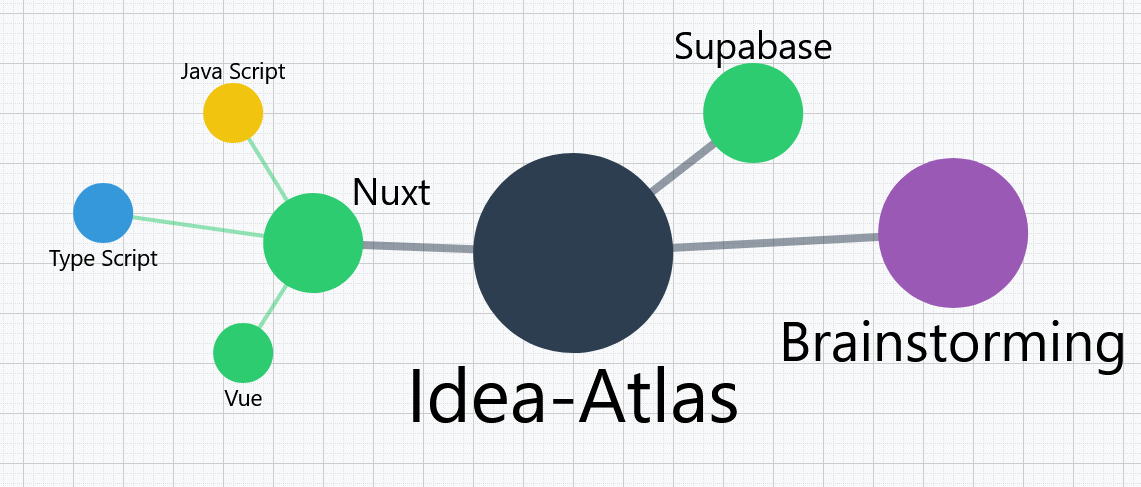
\includegraphics[width=1\linewidth]{Images/graph.png}
    \caption{Ukázkový graf}
    \label{fig:graph}
\end{figure}
\subsection{Konfigurace V-network-graph}
\label{config}
Konfigurace této knihovny hraje v mém projektu zásadní roli. Konfigurace se postupně měnila a rostla spolu s komplexitou projektu. Zejména se jedná o upravené, personalizované výtažky z dokumentace V-network-graph \cite{vnetexamples}. Kompletní konfigurační soubor \textit{mapNetworkConfig.ts} je k nalezení v adresáři \textit{config}.
\par
Na ukázce \ref{config1} se nachází první část konfigurace V-network-graph, konfiguruje se zde na příklad:
\begin{enumerate}
    \item zdali je povolen box selection a jak vypadá
    \item vzhled mřížky na pozadí
    \item vypnutí zvětšování objektů podle přiblížení
    \item minimální a maximální přiblížení, které může uživatel provést
    \item zakázání přiblížení při dvojitém kliku; v mém projektu má dvojtý klik funkci přidání nového uzlu
\end{enumerate}
\begin{lstlisting}[style=JavaScript, firstnumber = 56, caption={config/mapNetworkConfig.ts, první část konfigurace vNG},
label = {config1}]
view: {
    /...
      boxSelectionEnabled: true,
      selection: {
        box: {
          color: "#0000ff20",
          strokeWidth: 1,
          strokeColor: "#aaaaff",
          strokeDasharray: "0",
        },
      },
      grid: {
        visible: true,
        interval: 10,
        thickIncrements: 5,
        line: {
        //...
        },
        thick: {
          color: "#cccccc",
          width: 1,
          dasharray: 0,
        },
      },
      layoutHandler: new vNG.GridLayout({ grid: 10 }),
      scalingObjects: true,
      minZoomLevel: 0.1,
      maxZoomLevel: 16,
      doubleClickZoomEnabled: false,
    },
    /...
\end{lstlisting}
Na ukázce \ref{config2} se konfigurují vlastnosti a vzhled vrcholů:
\begin{enumerate}
    \item jak vypadá vrchol v normálním stavu
    \item jak se změní vrchol, když na něj uživatel najede myší
    \item jak vypadá popisek vrcholu; dále se tam zapíná automatické posouvání popisku, aby nepřekážel hranám, které vedou z daného vrcholu
\end{enumerate}
\begin{lstlisting}[style=JavaScript, firstnumber = 87, caption={config/mapNetworkConfig.ts, druhá část konfigurace vNG},
label = {config2}]
    node: {
      normal: {
        type: "circle",
        radius: node => node.size, // Use the value of each node object
        color: node => node.color,
      },
      hover: {
        radius: node => node.size + 4,
        color: node => node.color,
      },
      selectable: true,
      label: {
        visible: true,
        fontFamily: undefined,
        fontSize: node => calculateFontSize(node.size),
        lineHeight: 1.1,
        color: "#000000",
        margin: 4,
        direction: "south",
        directionAutoAdjustment: true,
        background: {
          visible: false,
          color: "#ffffff",
          padding: {
            vertical: 1,
            horizontal: 4,
          },
          borderRadius: 2,
        },
      },
    },
\end{lstlisting}
\newpage
Na ukázce \ref{config3} se nastavuje:
\begin{enumerate}
    \item zda se dají vybrat hrany
    \item jak vypadají hrany v normálním stavu
    \item co se stane s hranami, když na ně uživatel namíří myšítkem
    \item jak budou hrany vypadat, když je uživatel označí
\end{enumerate}
\begin{lstlisting}[style=JavaScript, firstnumber = 118, caption={config/mapNetworkConfig.ts, třetí část konfigurace vNG},
label = {config3}]
edge: {
      selectable: true,
      normal: {
        width: edge => edge.width, // Use the value of each edge object
        color: edge => convertToRGBA(edge.color),
      },
      hover: {
        width: edge => edge.width,
        color: edge => edge.color, // Use original color without transparency
      },
      selected: {
        width: edge => edge.width * 1.5, // Increase width by 50% when selected
        color: edge => edge.color,
        dasharray: "6",  // Fixed dash pattern for selected edges
        animate: true,   // Always animate selected edges
      },
    },
\end{lstlisting}


\section{Backend}
Vybral jsem si Supabase jako řešení backendu pro svůj projekt, protože nabízí open-source alternativu k Firebase s výkonnou PostgreSQL databází, která umožňuje flexibilní práci s daty, dále nabízí i bezplatný tier služby pro vývoj. Díky vestavěné podpoře pro autentizaci, realtime synchronizaci a serverless funkce poskytuje moderní a škálovatelné řešení bez nutnosti správy složité infrastruktury. Díky modulům se Supabase dobře integruje s Nuxt 3 a usnadňuje vývoj díky přehlednému API a skvělé dokumentaci.\cite{NuxtSupabase, supabasedocs}
\subsection{Ověření uživatele}
Supabase využívá tabulku \textit{auth.users} pro ověřování uživatelů, kterou spravuje automaticky. Když se někdo zaregistruje pomocí e-mailu a hesla, jeho účet se uloží do této tabulky. Zároveň mu systém automaticky odešle e-mail s potvrzovacím odkazem, který je nutné kliknutím ověřit, aby byl účet aktivován.\cite{supabseAuth, JohnKomarnicki}
\newline
Kromě toho Supabase podporuje i další metody autentizace, jako je přihlášení přes externí poskytovatele (např. Google, GitHub) nebo přihlášení pomocí magic linku, přičemž Supabase zajišťuje bezpečnost a šifrování citlivých údajů.\cite{supabseAuth} Bohužel kvůli zbytečné složitosti ze strany Googlu při přidání Google authenticatoru jsem se rozhodl zůstat pouze u e-mailu a klasického hesla.
\subsection{Middleware}
Middleware je software nebo kód, který funguje jako prostředník mezi různými částmi aplikace, například mezi klientem a serverem nebo mezi různými vrstvami v aplikaci. Obvykle se používá k manipulaci s požadavky a odpověďmi, autentizaci, logování, zpracování chyb nebo modifikaci dat předtím, než se dostanou k hlavní aplikaci. \cite{geeksforgeeks-2024}
\newline
V mém projektu slouží middleware k tomu, abych ověřil, zda je uživatel přihlášený, když se snaží dostat na části webové stránky, kde je to nutné; například na uživatelský profil.\cite{LearnVue}. Na ukázce \ref{middleware} je možné vidět jednoduchý kód, který ověří, zdali je uživatel přihlášen, a pokud není, přesměruje ho na login page.

\begin{lstlisting}[style=JavaScript, firstnumber = 1, caption={middleware/auth.js, middleware}, label={middleware}]
export default defineNuxtRouteMiddleware(() => {
    const user = useSupabaseUser();
    if (!user.value) {
        return navigateTo('/login');
    }
});}
\end{lstlisting}
Middleware pak jde snadno použít na libovolné stránce. Jeho názorné použití lze najít na ukázce \ref{middleware2}
\begin{lstlisting}[style=JavaScript, firstnumber = 2, caption={pages/profile.vue, ověření přihlášeného uživatele}, label={middleware2}]
definePageMeta({
    middleware: ["auth"],
});
\end{lstlisting}
\subsection{Struktura databáze}
Data jsou ukládána do 4 tabulek viz obrázek \ref{fig:scheme}. Tyto tabulky jsou propojené přes \textit{graph id}. Tedy každý node, edge a layout spadá pod nějaký graf.

\begin{figure}[h]
    \centering
    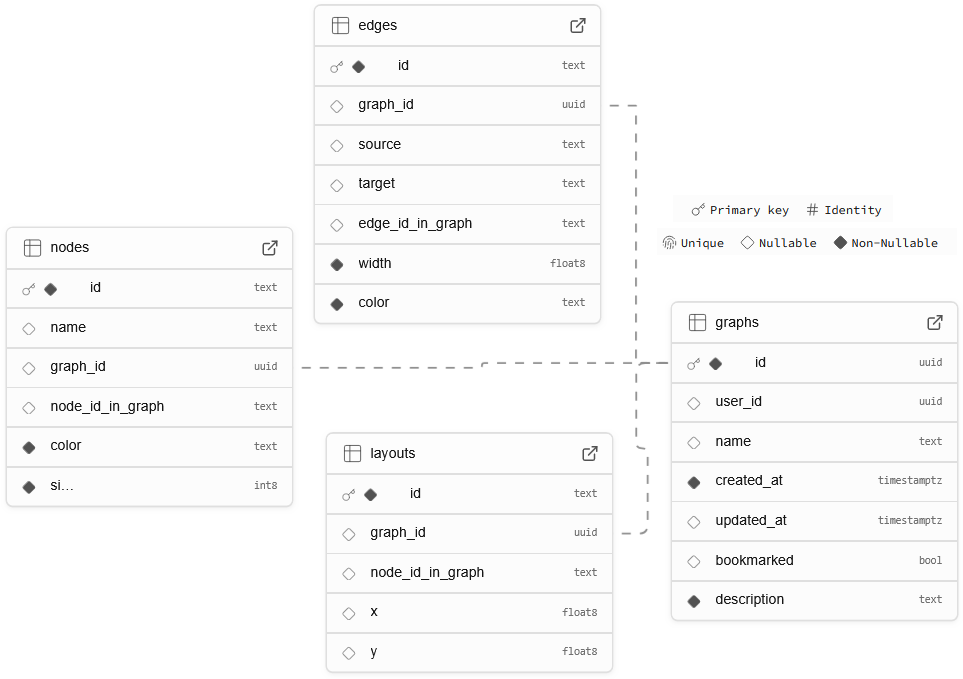
\includegraphics[width=1.1\linewidth]{Images/scheme.png}
    \caption{Schéma databáze}
    \label{fig:scheme}
\end{figure}
Za zmínku také stojí, že kvůli jednodušší implementaci s knihovnou v-network-graph, jsem se rozhodl pro propojení jednotlivých prvků grafu přes \textit{id in graph} a nikoliv propojení samotných tabulek pomocí cizího klíče. Jelikož každý node je ve v-network-graph grafové struktuře používán jako klíč, tak někdy i jako hodnota objektu viz ukázka \ref{mapping}. Tohle mé řešení sice není konvenční, nicméně mi to ulehčilo práci při mapování získaných dat z databáze.
\begin{lstlisting}[style=JavaScript, firstnumber = 1, caption={Demonstrace problému s mapováním}, label={mapping}]
// Ukazkova data
const nodes: Nodes = {
  node1: { name: "Rocket", color: "#2c3e50", size: 100 },
  node2: { name: "Fuel",color: "#2ecc71", size: 50  },
}
const edges: Edges = {
  edge1: { source: "node1", target: "node2", color: "#2c3e50", width: 8 },
}

\end{lstlisting}
\subsection{Dotazy do databáze}
Dotazy do databáze zařizují soubory \textit{graphService.js} a \textit{graphMetadataService.js}. Soubor \textit{graphService} se stará přímo o data konkrétního grafu. Kdežto \textit{graphMetadataService} se stará o metadata jednotlivých grafů, tedy posílá dotazy na jméno myšlenkové mapy, poslední datum editace a podobné.
\newline
Na ukázce \ref{dbrequest} je k nalezení část funkce \textit{fetchData}. Tato ukázka slouží jako demonstrace jednoduchého dotazu do databáze. Jako argument potřebuje objekt \textit{useSupabaseClient()} a id grafu, jehož data chceme dotazem získat.\cite{NetNinja1}

\begin{lstlisting}[style=JavaScript, firstnumber = 206, caption={utils/graphService.js, dotaz do databáze}, label={dbrequest}]
async function fetchData(supabase, graph_id) {
  const { data: nodesData, error: nodesError } = await supabase
    .from('nodes')
    .select('*')
    .eq('graph_id', graph_id);
  if (nodesError) throw nodesError;
}
\end{lstlisting}
\subsection{Row-level security}
RLS (Row-Level Security) jsou v Supabase bezpečnostní pravidla, která určují, kdo může přistupovat k jednotlivým řádkům tabulky v databázi. Supabase používá PostgreSQL Row-Level Security (RLS) k omezení přístupu na základě definovaných podmínek.\cite{RLC}
\newline
Na obrázku \ref{fig:RLC} je možné vidět RLC pro tabulku \textit{graphs} . Tato podmínka je vyhodnocována vždy při dotazu a danou akci databáze provede pouze, jestliže je pravidlo splněno. V tomto konkrétním případě může smazat user jenom svůj vlastní graf.
\begin{figure}[h]
    \centering
    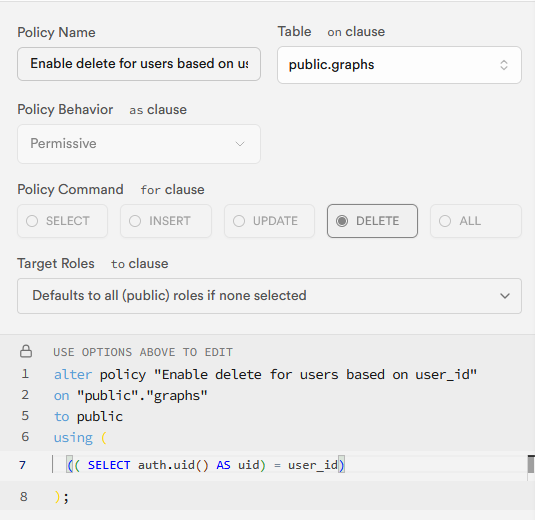
\includegraphics[width=0.6\linewidth]{Images/RLC.png}
    \caption{Příklad Supabase RLC}
    \label{fig:RLC}
\end{figure}
\subsection{Ukládání změn v grafu}
Na ukázce \ref{savegraph} je popsána funkce, která kompletně řeší problematiku uložení dat grafu. Nejprve pošle dotaz do databáze na získání všech ID pro daný graf. Následně vyfiltruje pouze ta ID, která jsou uložena v databázi, ale už ne lokálně v prohlížeči \cite{W3}; uživatel je tedy smazal. Pošle delete dotaz do databáze na tato vybraná data. Následně upsertne všechna data, která graf v prohlížeči obsahuje. Nová data jsou tedy přidána a změněná jsou updatnuta. Jde o jednoduché v celku elegantní řešení, které je konzistentní a spolehlivé.
\begin{lstlisting}[style=JavaScript, firstnumber = 168, caption={utils/graphService.js, uložení grafu}, label={savegraph}]
async function saveGraph(supabase, data, graph_id) {
  try {
    // Get current IDs from database
    const ids_in_db = await fetchAllIds(supabase, graph_id);
    
    // Find items to delete
    // __ is a placeholder for the layoutsToDelete variable - they are not used 
    const { nodesToDelete, edgesToDelete, __ } = await filterDeletedData(data, ids_in_db);
    // First delete edges
    await deleteEdges(supabase, edgesToDelete, graph_id);
    //....
    // Now upsert all current data
    await upsertGraphData(supabase, data, graph_id);
    
    // Update the graph's updated_at timestamp
    const { error: updateError } = await supabase
      .from('graphs')
      .update({ updated_at: new Date().toISOString() })
      .eq('id', graph_id);
}
\end{lstlisting}
\subsection{Automatické ukládání}
Při práci s interaktivními grafy je důležité zajistit, aby uživatelské změny byly automaticky ukládány, aniž by docházelo k nadměrnému zatěžování databáze. V komponentě \textit{MapNetwork.vue} je tato funkcionalita implementována pomocí debounce vzoru, který minimalizuje počet zbytečných požadavků na server a zároveň uchovává data uživatele v bezpečí. \cite{autosave}
\newline
Aby bylo možné efektivně reagovat na časté změny v grafu, využívá implementace časovou prodlevu mezi úpravou a samotným uložením. \textit{AUTO SAVE DELAY} je nastaven na 2 sekundy, což znamená, že pokud uživatel provede změnu, systém čeká, zda dojde k další úpravě. Teprve pokud během této doby žádná další změna nenastane, proběhne uložení.

Celý proces je řízen několika klíčovými prvky:
\begin{enumerate}
    \item \textit{saveTimeout} uchovává ID časovače, který řídí zpoždění ukládání.
    \item \textit{isSaving} sleduje, zda právě probíhá proces ukládání, což umožňuje zobrazit vizuální indikátor.
        
\end{enumerate}

Při každé změně v grafu je nejprve zrušen existující časovač, aby se zabránilo vícenásobnému ukládání. Poté se nastaví nový časovač, který po uplynutí definované prodlevy spustí funkci \textit{handleSave()}, jež provede uložení dat do Supabase.
\newline
Aby systém spolehlivě detekoval jakékoli změny, využívá Vue watcher, který sleduje uzly, hrany a rozložení grafu s nastavením deep: true. To znamená, že změny na jakékoli úrovni těchto objektů automaticky aktivují proces ukládání.
\begin{lstlisting}[style=JavaScript, firstnumber = 165, caption={components/MapNetwork.vue, automatické ukládání}, label={autosave}]
const saveTimeout = ref<NodeJS.Timeout | null>(null);
const isSaving = ref(false);

// Debounced auto-save function
const debouncedSave = () => {
  if (saveTimeout.value) {
    clearTimeout(saveTimeout.value);
  }
  
  saveTimeout.value = setTimeout(async () => {
    isSaving.value = true;
    try {
      await handleSave();
    } finally {
      isSaving.value = false;
    }
  }, AUTO_SAVE_DELAY);
};

// Watch for changes in data and trigger auto-save
watch(
  () => [data.nodes, data.edges, data.layouts],
  () => {
    debouncedSave();
  },
  { deep: true }
);
\end{lstlisting}
\section{Klíčové problémy}
Během mé práce jsem se setkal s mnoha problémy, spoustu z nich mělo jednoduché řešení, jiné byly o mnoho komplikovanější a zásadní pro mou vizi funkčnosti tohoto webového nástroje. V této kapitole jsou popsány ty nejvýznamnější z nich.
\subsection{Automatické uspořádání}
Chtěl jsem, aby Idea-Atlas disponoval funkcí automatického uspořádání vrcholů, tak aby vznikl na první pohled přehledný graf. Ukázalo se, že se jedná o velmi těžkou úlohu. Zprvu jsem se snažil přijít s vlastním algoritmem, ale to velmi rychle selhalo. Následně jsem se snažil na můj problém aplikovat \textit{Force-directed graph drawing} algoritmus \cite{wikiforce}; jde vcelku o komplexní algoritmy, bohužel má implementace selhala. Následně jsem zjistil, že v-network-graph má v sobě zabudované propojení s D3.js. Dohromady tak tyto 2 knihovny nabízejí konfigurovatelný force layout, který jsem metodou pokus-omyl nastavil.
\begin{lstlisting}[style=JavaScript, firstnumber = 32, caption={config/mapNetworkConfig.ts, Implemetnace force layout},
label = {force}]
export const ForceConfig = new ForceLayout({
  positionFixedByDrag: false,        // Nodes continue simulation after being dragged
  positionFixedByClickWithAltKey: true,  // Alt+Click fixes node position
  createSimulation: (d3, nodes, edges) => {
    // Create links between nodes with specified parameters
    const forceLink = d3.forceLink<ForceNodeDatum, ForceEdgeDatum>(edges)
      .id((d: { id: any; }) => d.id)  // Use node's id property to establish connections
    
    return d3
      .forceSimulation(nodes)
      // Edge force: maintains distance between connected nodes
      .force("edge", forceLink.distance(FORCE_LINK_DISTANCE).strength(FORCE_LINK_STRENGTH))
      // Charge force: makes nodes repel each other
      .force("charge", d3.forceManyBody().strength(FORCE_CHARGE_STRENGTH))
      // Center force: pulls nodes toward canvas center
      .force("center", d3.forceCenter().strength(FORCE_CENTER_STRENGTH))
      .alphaMin(FORCE_ALPHA_MIN)  // Minimum energy level before simulation stops
  }
});
\end{lstlisting}
\newpage
Force layout automaticky a dynamicky simuluje přitažlivé síly jednotlivých hran a odpudivé síly vrcholů, výsledkem je přehledné uspořádání grafu, viz obrázky \ref{fig:chaos} a \ref{fig:order}. Uživatel si může přepínat mezi normálním grid layoutem nebo mezi force layoutem. 
\begin{figure}[h]
    \centering
    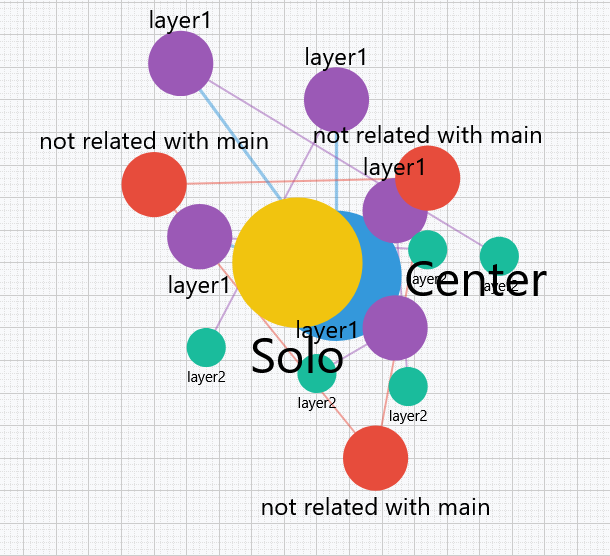
\includegraphics[width=0.6\linewidth]{Images/Chaos.png}
    \caption{Chaotické uspořádání vrcholů}
    \label{fig:chaos}
\end{figure}
\begin{figure}[h]
    \centering
    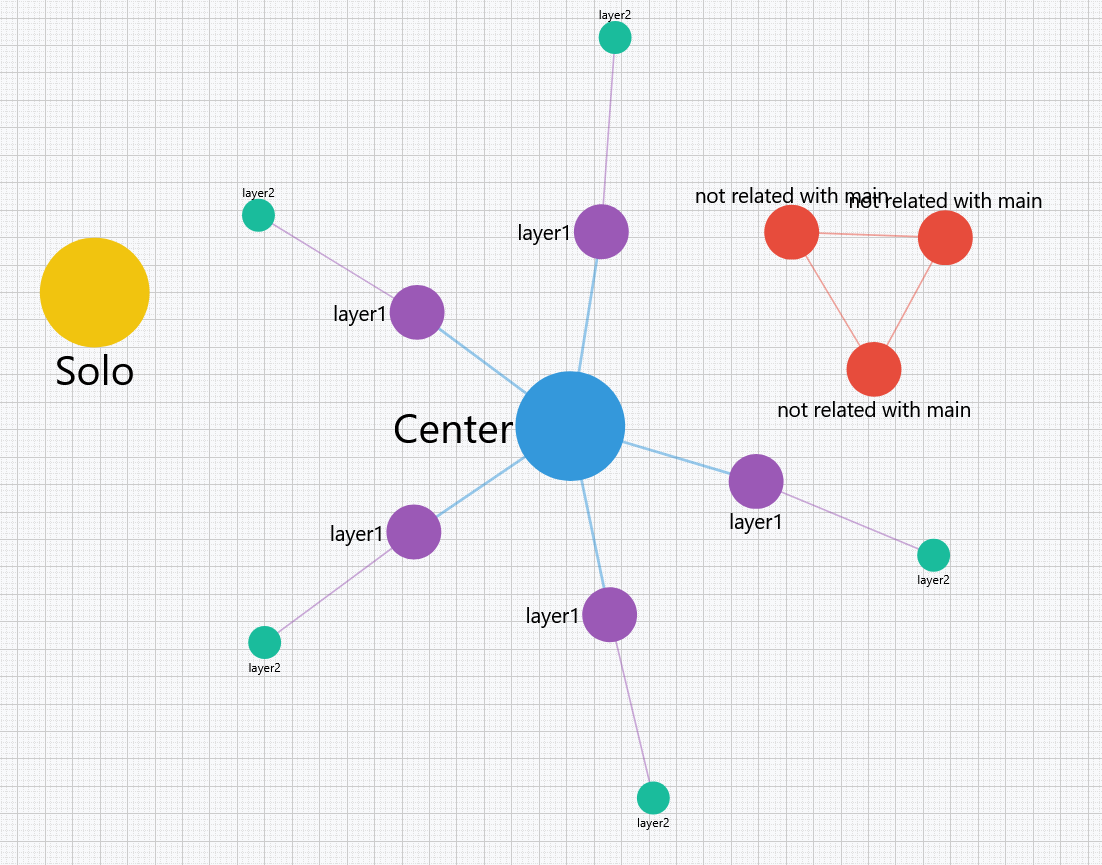
\includegraphics[width=0.7\linewidth]{Images/ordered.png}
    \caption{Uspořádání po použtí force layout}
    \label{fig:order}
\end{figure}
\newpage
\subsection{Historie editací}
 K správě historie editací je používán soubor \textit{graphHistory.js}. Obsahuje jednu třídu \textit{HistoryManager}. Je založena na hlavním poli \textit{history}, elementy tohoto pole jsou kopie dat grafu v určitý okamžik. Historie může mít celkem až 100 záznamů (aby nedošlo k zbytečnému plýtvání pamětí). Dále je zde index, jenž určuje aktuální polohu v historii. 
\begin{lstlisting}[style=JavaScript, firstnumber = 4, caption={utils/graphHistory.js, proměné třídy HistoryManager},
label = {HM}]
class HistoryManager {
    constructor() {
        this.history = [];
        this.currentIndex = -1;
        this.maxHistory = HISTORY_MAX_LENGTH; // Maximum number of saved states
    }
\end{lstlisting}
Při každé změně dat grafu (například při přidání nového vrcholu) se udělá jejich kopie a přidá se do historie. Následně se smaže veškerá budoucí historie; jde o případ, kdy jsme se nejdříve vrátili do minulosti a pak provedly nové úpravy - tedy tu minulé musí být odstraněny. Následně zvětšíme index současného bodu v historii  a pokud jsme přesáhli velikost historie, jsou data posunuta směrem na začátek a první záznam je smazán a index současnosti je zmenšen o jedna.
\begin{lstlisting}[style=JavaScript, firstnumber = 13, caption={utils/graphHistory.js, přidání do historie},
label = {historyadd}]
addToHistory(data) {
        // Create deep copy using structuredClone
        const dataCopy = {
        // .....
        };
        // Remove any future history entries
        this.history = this.history.slice(0, this.currentIndex + 1);

        this.currentIndex++;
        this.history[this.currentIndex] = dataCopy;
        // If currentIndex is greater than maxHistory, remove the first element
        // And shift all elements to the left
        if (this.currentIndex > this.maxHistory) {
            this.history.shift();
            this.currentIndex--;
        }
    }
\end{lstlisting}
\subsection{Převod sousřadnic mezi SVG a DOM}
Aby program věděl, kde se má zobrazit dialog pro vytvoření vrcholu nebo jeho editaci. Musel jsem převést souřadnice z SVG souřadnicového systému (tedy toho, co používá vNG) do DOM souřadnicového systému (souřadnice v okně prohlížeče).\cite{coords}
\begin{lstlisting}[style=JavaScript, firstnumber = 385, caption={components/MapNetwork.vue, převod z Svg souřadnic do Dom},
label = {coords}]
 // Translate from SVG to DOM coordinates
const domPoint = graph.value.translateFromSvgToDomCoordinates({ x: nodeLayout.x, y: nodeLayout.y });
\end{lstlisting}
Dále byla potřeba omezit, kde až se může dialog objevit. Například by nebylo přehledné a intuitivní, kdyby se dialog objevil příliš nahoře a nebyl by tak tedy vidět. Funkce posune souřadnice dolů, nahoru, doleva nebo doprava, podle vzájemné pozice od okrajů okna v prohlížeči, viz ukázka \ref{offset}. \cite{windowsize}
\begin{lstlisting}[style=JavaScript, firstnumber = 395, caption={components/MapNetwork.vue, výpočet offset dialogu},
label = {offset}]
  const windowWidth = window.innerWidth;
  const windowHeight = window.innerHeight;

  // Calculate horizontal offset
  let xOffset = domPoint.x < windowWidth / 2 ? DIALOG_WIDTH/2 + PADDING : -(DIALOG_WIDTH/2 + PADDING);
    
    // Calculate vertical offset
  let yOffset = 0;
  if (domPoint.y < DIALOG_HEIGHT + PADDING) {
    // Too close to top - move down
    yOffset = (DIALOG_HEIGHT/2 + PADDING) - domPoint.y;
  } else if (domPoint.y > windowHeight - DIALOG_HEIGHT - PADDING) {
    // Too close to bottom - move up
    yOffset = (windowHeight - DIALOG_HEIGHT/2 - PADDING) - domPoint.y;
  }
  
  return {
    x: domPoint.x + xOffset,
    y: domPoint.y + yOffset
    };
\end{lstlisting}
\newpage
\subsection{Správa UI stavů}
Další důležitý problém, který bylo potřeba vyřešit, bylo, jak správně spravovat stavy UI. Například jak zařídit, aby se nesmazal vrchol, když klávesou \textit{backspace} smažu znaky při editaci jména vrcholu. Vytvořil jsem samotný soubor \textit{uiTracker.ts} ve složce \textit{utils}, který kontroluje jednotlivé UI komponenty, zdali nejsou otevřené. Implementace je velice jednoduchá, za to účinná a přehledná.
\subsection{Přetahovatelné UI}
\textit{useDraggable.ts} umožňuje přetahování HTML prvků. Poskytuje funkci \textit{startDrag}, která se stará o výpočet počáteční pozice, správu událostí myši a aktualizaci pozice prvku. Po kliknutí na prvek se určí jeho aktuální souřadnice a vypočítá se posun mezi místem kliknutí a jeho skutečnou polohou. Během přetahování se aktualizují CSS vlastnosti \textit{style.left} a \textit{style.top}, přičemž \textit{callback onPositionChange} umožňuje sledování nových souřadnic, viz ukázka \ref{drag}. Jakmile uživatel pustí tlačítko myši, obslužné funkce pro pohyb a ukončení přetahování se odstraní, aby nedocházelo k nežádoucím interakcím. Tento hook poskytuje jednoduché a efektivní řešení pro přetahování prvků v rámci Vue komponentů.\cite{draggable}
\begin{lstlisting}[style=JavaScript, firstnumber = 1, caption={utils/useDraggable.ts, přetahovatelné UI},
label = {drag}]
export function useDraggable() {
  const startDrag = (event: MouseEvent, element: HTMLElement,
  onPositionChange: (x: number, y: number) => void) => {
    // Calculate the initial position from the element's current position
    const currentX = parseInt(element.style.left) || 0;
    const currentY = parseInt(element.style.top) || 0;
    
    // Calculate the offset from where we clicked relative to the current position
    const offsetX = event.clientX - currentX;
    const offsetY = event.clientY - currentY;

    const handleMove = (moveEvent: MouseEvent) => {
      const newX = moveEvent.clientX - offsetX;
      const newY = moveEvent.clientY - offsetY;
      
      element.style.left = `${newX}px`;
      element.style.top = `${newY}px`;
      onPositionChange(newX, newY);
    };// ....
\end{lstlisting}
\input{Kapitoly/10Návrhy}
\section{Závěr}
Idea-Atlas je komplexní projekt s důrazem na detail. Na projektu jsem pracoval průběžně a strategicky jsem si jeho vyhotovení rozvrhl.
\newline
Zadání se mi podařilo téměř celé splnit. Vytvořil jsem plně funkční webovou aplikaci, která slouží jako přehledný a snadno ovladatelný nástroj pro tvorbu myšlenkových map. Bohužel se mi ze zmíněných důvodů nepodařilo implementovat ChatGPT API, a aplikace tak neumožňuje automatickou generaci pojmů a jejich závislostí. Podařilo se mi úspěšně nalézt i použít moderní technologie hodící se pro řešení zadané problematiky. Celkově vnímám Idea-Atlas jako velmi přínosný projekt, který mi pomohl prohloubit znalosti a posunout se dál nejen v oblasti vývoje webových aplikací.

\section{Použité zdroje}

\printbibliography[heading=none]

\newpage
\mbox{}
\addcontentsline{toc}{section}{\listfigurename}
\listoffigures
\newpage
\mbox{}
\addcontentsline{toc}{section}{Seznam ukázek kódu}
\lstlistoflistings

\end{document}
